%
%   K A D O N O
%   "kadono.tex"
%

\documentclass[10pt,b5paper,papersize,dvipdfmx]{jsbook}

\usepackage{vuccaken}
\usepackage{vuccaken2019}

% スタイルファイルの読み込みや自作マクロは、
% 最終的には vuccaken2019.sty の中に書いてください。
% とりあえずはここに書いてもらって構いません。


\begin{document} % 以下本文

% \mokuji{2} % 目次出力

% - - - - - - - - - - - - - - - - - - - - - - - - %
\kaishititle%
  {温度の子}% title
  {基礎理工学研究科M1回生}% 所属
  {\vname{門野}{広大}}% name
% - - - - - - - - - - - - - - - - - - - - - - - - %


\section*{はじめに}
熱って何?温度ってなに?どうやって熱は伝わっているの?そんな疑問に一生に一度は出会ったことがあると思います。実際熱の伝わり方というものをちゃんと理解しようとすると莫大な時間がかかりますし、不可逆なものでもあるのでそもそも理解できないのかもしれません。でも、限定的な条件において理解することは容易にできます。今回の会誌ではそんな物理の世界では常識的なことを主に書いていきたいと思います。\par
今回は状況が限定的な状態で、実際に人間が住んでいる環境とはかけ離れているため役に立たないと思われると思います。研究分野ではとても役にたちます。その理由を最後の方に私がやっている研究の話を含めて書きたいと思います。

% 熱って何?そもそも温度って何?熱伝導率って何で決まるの?物質のなに?格子ってなに?
% 格子振動って何?フォノンってなに?

%
\section{温度}
温度とは、辞書で検索すると「温冷の度合いを表す指標である」と書いてあります。その通りなんですけど、状態量として使われているので、そもそもどういう形で決まっているのか気になると思います。私は今回この会誌を書くに当たってとても気になりました。\par 
普段日本人なら$^\circ \rm{C}$という単位の世界で過ごしていると思います。これはセルシウス度というものらしいです。水を冷やしていったときに氷になる温度を$0 ^\circ \rm{C}$として、水を温めていったときに沸騰する温度を$100 ^\circ \rm{C}$と決めた温度だそうです。ほかにもいろんな温度があるらしいですが、今回使う温度の単位は$\rm{K}$です。高校の物理でもやると思うので知っている人は多いと思いますが、読み方はケルビンです。このケルビンは国際単位系で熱力学温度の単位になっています。\par





ケルビンが何を基準にしているのかを考える前に、温度というものはミクロの世界で考えるとどういうものに対応するのかということを考えていきましょう。統計力学の教科書を読むと物質を構成する分子がもつエネルギーの統計値である、と書いてあります\par





絶対温度はほかの状態量の中で測定するがかなり難しいです。実際に大学の研究室で試料の温度を測定するときに使用している温度計はいろんな種類がありますが、その中の一つはセルノックス温度センサーです。私も実際に実験で使用しました。この温度計は温度が上がると抵抗値が下がるという負の温度係数を持っています。
\begin{figure}[htbp]
  \begin{center}
      \begin{tabular}{c}
      % 1
      \begin{minipage}{0.5\hsize}
          \begin{center}
          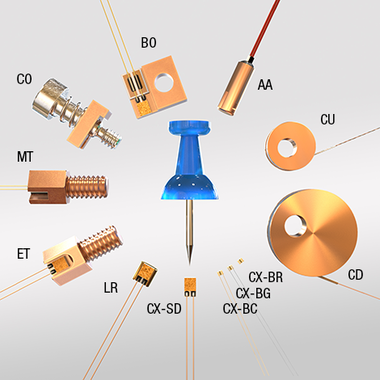
\includegraphics[clip, width=4.2cm]{img/cryotronics.png}
          % \hspace{1.6cm} [A]\ セルノックス温度センサ
          \end{center}
      \end{minipage}
      % 2
      \begin{minipage}{0.5\hsize}
          \begin{center}
          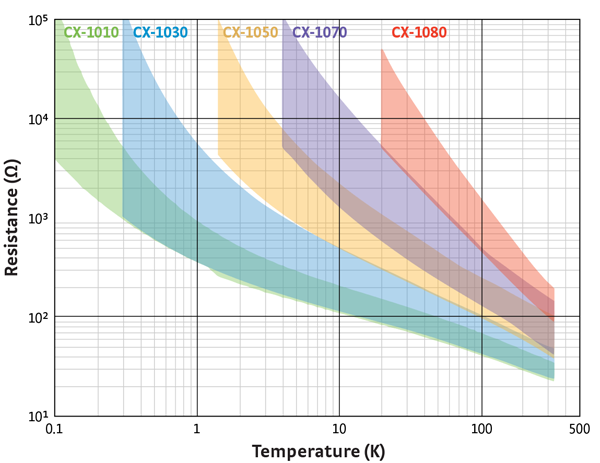
\includegraphics[clip, width=5cm]{img/CX-chart-1.png}
          % \hspace{1.6cm} [B]\ センサーの抵抗温度特性
          \end{center}
      \end{minipage}
  
      \end{tabular}
      \caption{左:セルノックス温度センサの外観、右:センサの温度依存性、参考文献\cite{ondo}より}
      \label{fig:cryotronics}
  \end{center}
\end{figure}

セルノックス温度計の大きさは図\ref{fig:cryotronics}の左側の写真にある通りとて小さいです。セルノックスは低温特に数ケルビンの極低温領域に強い温度計です。摂氏でいうと$-270\ ^\circ \rm{C}$付近です。図\ref{fig:cryotronics}の右のグラフはセルノックスの温度と抵抗値の特性をのせています。色の違いは種類の違いです。このグラフを見ると温度と抵抗値のグラフが直線ではなく幅を持っています。これはセルノックスの温度計自体にこれだけの抵抗値の誤差があるということではありません。個体差がこれくらいの幅を持っているということです。この温度計を買うとものと一緒に温度と抵抗値のデータがついてきます。このデータは企業側が測定してくれたデータです。このデータを使って校正することによって温度を正確に測定することができます。というように、絶対温度を測定するのは難しくどうしても相対温度を測定することになってしまいます。\par
温度はどういうものでどう測定しているのかについてほんとふわっと理解できたと思います。では、ここからいよいよ固体中に存在している温度の子とも言えそうな粒がいるということを考えていきたいと思います。

\section{フォノン君}
今回は気体、液体ではなく、固体の中の熱の流れについて考えようと思います。
\subsection{格子振動}
まず考えたいのが、固体の中でも、一つの原子のみで構成されている単結晶です。
最初から三次元で考えるとよくわからなくなるので、原子同士がばねで一列につながっている状態を考えます(図\ref{fig:bane})。\par


\begin{figure}[htbp]
  \centering
  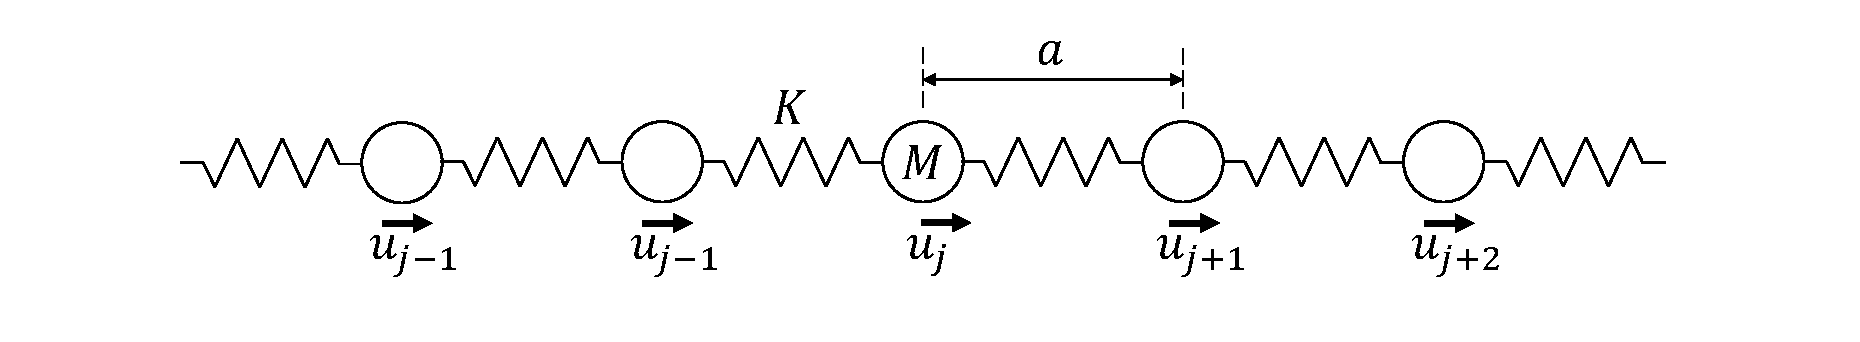
\includegraphics[height=2cm]{img/bane.pdf}  % width
  \caption{一次元の結晶}
  \label{fig:bane}
\end{figure}
構成原子は最近接の間にだけ力を及ぼし会うと仮定します。$s$番目の原子の変位を$u_s$すると、$s$番目の原子の運動方程式は次のようになります。。
\begin{align}
  M\frac{\mathrm{d}^2u_s}{\mathrm{d}t^2} = F_s = K (u_{s+1} - u_s) - K (u_s - u_{s-1})
  \label{eq:satom}
\end{align}
ここで、$M$は原子の質量、$\alpha$はばね定数、$F_s$は$s$番目の原子に及ぼす力。\par
式\ref{eq:satom}の解は波の式であると予測されます。波の式について少し話をしましょう。代表的な正弦波をあらわす式は
\begin{align}
  A(x) = A_0 \sin \left(\frac{2\pi x}{\lambda} + \phi \right)
\end{align}
とかけます。\par
ここで、波数$k$というものを導入すると、
\begin{align}
  A(x) = A_0 \sin (kx + \phi)
\end{align}
となります。波数$k (= 2\pi/\lambda)$は、単位長さあたりに含まれる1波長分の波の数に$2\pi$をかけた量である。さあ、ここで波数$k$というものをわざわざ導入しました。どうしてこんなものを導入するのか疑問に思う人がいると思います。大学では友達以上にであう波数$k$がどういうものを示しているのでしょうか。この波数$k$というものは距離を位相に変換するツールの役割をしています。つまり、この波数$k$というものを用いることによって空間における波の変動を記述することができます。波数という概念はいろんなものを記述できるので物理の世界ではめっちゃ使います。\par
この波数が波の進行方向を含んだ波数ベクトル$\bm{k}$という形にして、空間波の式は次のようになります。
\begin{align}
  u(\bm{r},t) = u_0 \exp(i(\bm{k} \cdot \bm{r} - \omega t))
\end{align}
ここで、$u_0$は振幅、$\bm{k}$は波数ベクトル、$\bm{r}$は位置ベクトル、$\omega$は角周波数。\par
今回は一次元を考えているので、式\ref{eq:satom}の解として次のような進行波を予想します。
\begin{align}
  u_s = u_0 \exp\{i(ska - \omega t)\}
\end{align}
これを、式\ref{eq:satom}に代入すると、
\begin{align}
  -M\omega^2 &= K\{\exp(ika) + \exp(-ika) - 2\} \\
             &= -2K\left(1-\frac{\exp(ika) + \exp(-ika)}{2}\right) \\
             &= -2K(1-\cos ka)\\
             &= -4K\sin^2\frac{ka}{2}
\end{align}
したがって、角振動数$\omega$と波数$k$の関係には次のような関係が導けます。
\begin{align}
  \omega = 2 \sqrt{\frac{K}{M}} \left| \sin \frac{ka}{2}\right|
\end{align}
上の式のグラフを図\ref{fig:bunnsan}に示す。
\begin{figure}[htbp]
  \centering
  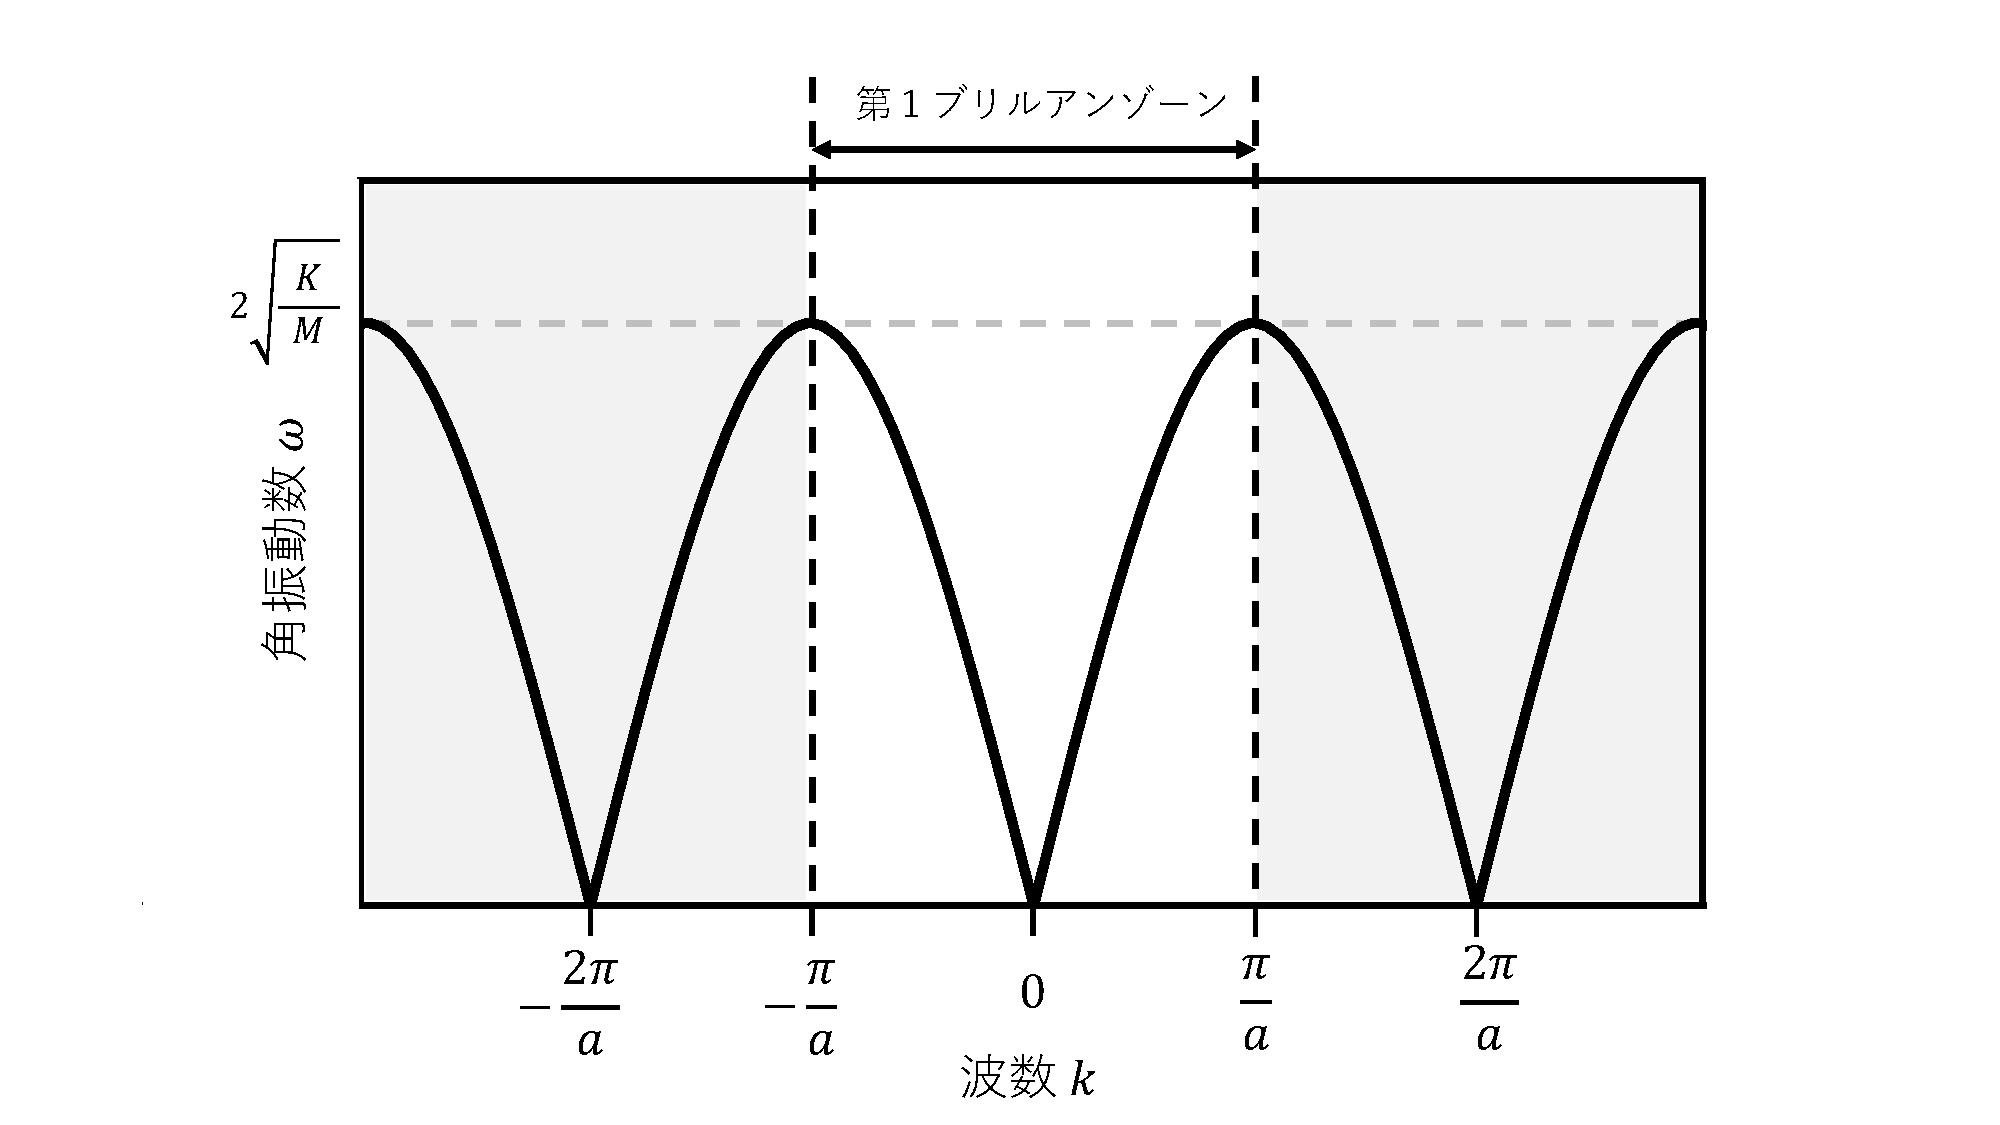
\includegraphics[width=10cm]{img/bunsann.pdf}  % width
  \caption{分散関係}
  \label{fig:bunnsan}
\end{figure}
この$\omega$と$k$の関係は分散関係と呼ばれます。この分散関係を見るといろんなことがわかります。図\ref{fig:bunnsan}を見ると明らかなように周期関数になっています。ある$k_r$に対して周期$\frac{2\pi}{a}$分だけ大きな波数$k_r' = k_r + \frac{2\pi}{a}$に対す解を求めると
\begin{align}
  u_s &= u_0 \exp\{i(sk_r'a - \omega t)\}\\
      &= u_0 \exp \left[i\left\{s \left(k_r + \frac{2\pi}{a}\right)a-\omega t\right\}\right]\\
      & = u_0 \exp {i(sk_ra + 2s\pi - \omega t)}\\
      & = u_0 \exp {i(sk_ra -\omega t)}
\end{align}
となり、波数$k_r$の場合の解と一致する。つまり、周期$\frac{2\pi}{a}$で繰り返して結局同じ解になるので分散関係については1周期分だけを考えれば十分である。この1周期を$-\frac{2\pi}{a} < k\leq \frac{2\pi}{a}$をとることが多いです。この範囲を第1ブリルアンゾーンと相当します。ブリルアンゾーンについてはここではあんまり関係ないので聞き流してください。\par
ここでもう少し図\ref{fig:bunnsan}について詳しく見ていきたいと思います。波数$k$が$0$に近い領域、つまり長波長の範囲($ka \ll 1$)では、$\sin \frac{ka}{2} \simeq \frac{ka}{2}$であることから、
\begin{align}
  \omega = a \sqrt{\frac{K}{M}}k
\end{align}
と近似することができる。つまり$\omega$と$k$は比例している。比例定数(グラフの傾き)について注目すると
\begin{align}
  \frac{\omega}{k} =a \sqrt{\frac{K}{M}}= \frac{2\pi\nu}{2\pi/\lambda} = \nu \lambda = v
\end{align}
であるので、グラフの傾きは音速$v$になります。今回求めた格子振動のモードを音響モードと呼びます。

\subsection{量子化}
量子力学によると、すべてのものは粒子と波の二重性を示すらしいです。この考えを今回の格子振動に適用して、粒子として考えることができます。この粒子のことをフォノン(phonon)と言います。\par
量子化について詳しく話したいと思っていたのですが、自分が予想以上に理解していないのとそもそも量子力学は理解できないものだと気が付いたので調和振動子のエネルギーの話だけ考えます。各振動数$\omega$の調和振動子のエネルギー$E$は
\begin{align}
  E = \left(n + \frac{1}{2}\right)\hbar \omega
\end{align}
であらわせます。ここで$n$は0以上の整数、$\hbar$はプランク定数を$2\pi$で割ったものです。これについて補足すると、$n = 0$のときでもエネルギーはゼロにならないこのエネルギーを零点エネルギーと解釈されています。粒子的な観点からこれをフォノンの個数に相当すると考えます。







\section{比熱とか熱伝導率とか}
ここからは、固体中の熱物性、特に比熱、熱伝導率、について書いていきたいと思います。ここからは統計力学の知識が必要ですが、それは参考文献に任せます。これから固体の熱物性について考えるに当たって固体の内部エネルギーを考えます。固体の内部エネルギーは、格子振動のエネルギーと電子系のエネルギーからなるのですが。格子振動のエネルギーに比べると、電子系のエネルギーは温度による変化が小さいため電子系のエネルギーの比熱への寄与は小さいです。
したがって今回は電子系のエネルギーについてはあまり考えずに格子振動についてのエネルギーについてをメインに扱います。
\subsection{比熱}
比熱について、まず比熱とは、1 kgの物質の温度を1 Kだけあげるのに必要な熱量として定義されます。水の場合、比熱は$4.2 \times 10^3\  \mathrm{J\ K ^{-1} kg^{-1}}$なので、1 kgの水の温度を1 Kあげるためには$4.2 \times 10^3 J$だけの熱量が必要ということになります。これに対して、銅の比熱は$3.8 \times 10^2\ \mathrm{J\ K ^{-1} kg^{-1}}$と水の比熱の1/10以下です。つまり、銅の方が水よりも10倍温まりやすいということがわかります。\par
ここからは、ミクロな視点で比熱を求めます。$N$原子系からなる格子振動のエネルギー$U$は
\begin{align}
  U = \sum_{\bm{k}}\sum_{q}\left(n_{\bm{k},q} + \frac{1}{2}\right)\hbar \omega_{\bm{k},q}
  \label{eq:nemui}
\end{align}
ここで、$\bm{k}$はフォノンの波数ベクトル、$q$はフォノンのモードの種類を示す\footnote{フォノン君の章では1次元のみを考えたため一つのモードしか出てこなかったが、3次元に拡張して考えると3の自由度があるため、三個のモードがある。縦モード(LA)1つ、横モード(TA)2つ}。比熱について考えるとき内部エネルギーがどのような温度依存性を示すかを考える必要があります。式\ref{eq:nemui}で温度変化するのは、フォノンの個数である$n_{\bm{k},q}$です。フォノンの個数が$n$である確率$P_n$は$\exp\left(-\frac{E}{k_BT}\right)$に比例するので、フォノンの個数の期待値は、
\begin{align}
  \left\langle n_{\bm{k},q}\right\rangle = \frac{\sum_{n = 0}^\infty nP_n}{\sum_{n = 0}^\infty P_n} = \cdots = \frac{1}{\exp \left(\frac{\hbar \omega_{\bm{k}, q}}{k_BT}-1\right)}
\end{align}
物質の温度を$\Delta T$あげるのに必要な熱量が$Q$であるとき、温度$\Delta T$上昇することによる物質の内部エネルギーの増加分は$\Delta U = Q$となるので、比熱$C$は、$\Delta T \rightarrow 0$の極限を求めることによって求めることができる。
\begin{align}
  C &= \lim_{\Delta T \rightarrow 0} \frac{Q}{\Delta T} = \lim_{\Delta T \rightarrow 0} \frac{\Delta U}{\Delta T} = \pdv{U}{T}\\
    &= \pdv{x} \sum_{\bm{k}}\sum_{q}\frac{\hbar \omega_{\bm{k},q}}{\exp\left(\frac{\hbar \omega_{\bm{k},q}}{k_BT}-1\right)}
\label{eq:totemonemutai}
\end{align}
格子比熱の式を求めることができた。
\subsubsection*{デバイモデル}
式\ref{eq:totemonemutai}で求める求めた格子比熱の式のままでは比熱の温度依存性や物質による比熱の違いなど具体的なことについては考察できない。様々な近似の方法はありますが、今回は低温の比熱について説明することができるデバイモデルについて考えていきます。\par
分散関係が$k = 0$付近では、$\omega_q = v_q k$と近似することができました。このデバイモデルは、全域で成り立つという仮定をしたモデルのことを言います。ここで、モードの違いで音速はすべて同じと仮定し、モードの種類は気にしないこととする。したがって式\ref{eq:totemonemutai}は、
\begin{align}
  C &= \pdv{T} \frac{3V}{(2\pi)^3} \int\frac{\hbar v k}{\exp \left(\frac{\hbar v k}{k_BT}\right)-1 }\dd{\bm{k}}\\
  & = \frac{3V}{(2\pi)^3} \int \frac{\hbar^2 v^2 k ^2}{k_B T ^2}  \frac{\exp \left(\frac{\hbar v k}{k_BT}\right)}{\left\{\exp \left(\frac{\hbar v k}{k_BT}\right)-1 \right\}^2}\dd{\bm{k}}\\
  &= \frac{3V}{(2\pi)^3} \int \frac{\hbar^2 v^2 k ^2}{k_B T ^2}  \frac{\exp \left(\frac{\hbar v k}{k_BT}\right)}{\left\{\exp \left(\frac{\hbar v k}{k_BT}\right)-1 \right\}^2} 4 \pi k^2 \dd k\\
  &= \frac{3V}{2\pi^2} \int \frac{\hbar^2 v^2 k ^4}{k_B T ^2}  \frac{\exp \left(\frac{\hbar v k}{k_BT}\right)}{\left\{\exp \left(\frac{\hbar v k}{k_BT}\right)-1 \right\}^2}  \dd {k}
  \label{eq:daigakutoutyaku}
\end{align}
となる。ここで、被積分関数は逆格子空間において、原点を中心に球対称になることを使って1変数の$k$についての積分に置き換えている。\par
この積分は逆格子空間の基本単位胞にわたって行うべきであるが、デバイモデルでは格子振動の各振動数の上限をデバイ各振動数$\omega_D$としている。







\begin{align}
  \Theta_D = \frac{\hbar \omega_D}{k_B}
\end{align}
この条件を利用して積分範囲を半径$k_D=\frac{\omega_D}{v} = \frac{k_B\Theta_D}{\hbar v}$内の球の内部に変更する。\par
この仮定の下で、$x = \frac{\hbar v k}{k_B T}$として変数変換すると、 式\ref{eq:daigakutoutyaku}は
\begin{align}
  C = 9Nk_B\left(\frac{T}{\Theta_D}\right)^3\int_0^{\Theta_D/T}\frac{x^4\mathrm{e}^x}{(\mathrm{e}^x -1)^2}\dd{x}
\end{align}
となる。\par
極低温領域($T \ll \Theta_D$)では、積分範囲の上限を$\infty$であると近似し、さらに
\begin{align}
  \int_0^\infty \frac{x^4 \mathrm{e}^x}{(\mathrm{e}^x-1)^2}\dd{x} = \frac{4\pi^4}{15}
\end{align}
であることを用いると
\begin{align}
  C &= \frac{12\pi^4}{5}Nk_B\left(\frac{T}{\Theta}\right)^3 \\
  &\propto T^3  
\end{align}
となる。固体の比熱は温度の$T$の3乗に比例して増加する。この結果は実験結果ととてもよく一致しており、大体の結晶でこのデバイの$T^3$則に従うことが知られている。
\subsection{熱伝導率}
今までは、調和近似のみで実際の実験結果を理解することができました。しかし、熱伝導率は、そのような調和近似だけでは理解できない、つまり非調和効果も考慮する必要がある。熱伝導率$\sigma_t$は
\begin{align}
  Q = \sigma_t \pdv {T}{x}
\end{align}
で定義される。ここで$Q$は$x$方向に垂直な単位断面積を通って、単位時間に流れる熱エネルギーである。\par
今回この熱伝導率について詳しく調べてまとめたいと思っていたのですが、会誌の原稿の締切が押し迫ってしまったので、低温における熱伝導率について少し話をしとくだけにしときます。気体分子運動論の処方にしたがって、フォノンの平均速度を$\overline{v}$、平均自由行程を$l$とすると、熱伝導率は次のように導くことができます。
\begin{align}
  \sigma_t = \frac{1}{3}l\overline{v}C
\end{align}
となります。\par
この式に基づいて低温での温度依存性について考えます。まずこの式で温度依存性について考えると、平均自由行程の温度依存性について考えます。平均自由行程は温度が低くなると次第に増加していくが、極低温領域で不純物どうしの平均距離などにより頭打ちとなり一定になります。次に比熱の温度依存性は先ほど比熱のセクションで説明した通り、$T^3$に比例して減少していきます。したがって、熱伝導率の温度依存性は低温では比熱の温度依存性が効いてくるため$T^3$に比例して減少します。

\section{ちょっと変わった話}
結晶において低温の熱物性について考えて来ました。前のセクションでいった温度依存性がすべての結晶でいえるのかというと実は例外があります。私の研究テーマになっているのですが、単結晶であってもなぜか結晶とは違う温度依存性を持つ物質がこの世の中には存在しています。リラクサー強誘電体というものです。
この物質は強誘電体の一種なのですが、詳しく説明すると一つ会誌ができてしまうのでここでは簡単に説明します。まず、誘電率というのは絶縁体の一種というか絶縁体です。大学入試とかでコンデンサの電気容量とかを計算した経験はあると思います。コンデンサに挟まっている種類の一つです。そのほかにもこの世界に生きているすべての人が持っているであろうスマートフォンの中にも強誘電体が入ってます。この強誘電体という物質は実は温度変化させると急激に変な変化する温度点があります。この温度は常温ではなく人が住めないくらいの温度域にあります。そのためスマートフォンなどの室温で使う機器などにはそこまで問題ありませんが、例えば人工衛星などの過酷な環境から室温まで同じように動かしたいときとかにかなり問題になります。そこで、急激な温度変化がないような物質がこの世の中にあってその物質の名前は「リラクサー強誘電体」というものです。この物質は温度変化に対してとても緩やかな変化をする物質です。種類によっては、とてもいい特性を持っていたりします。
\begin{figure}[htbp]
  \begin{center}
      \begin{tabular}{c}  
      \begin{minipage}{0.5\hsize}
          \begin{center}
            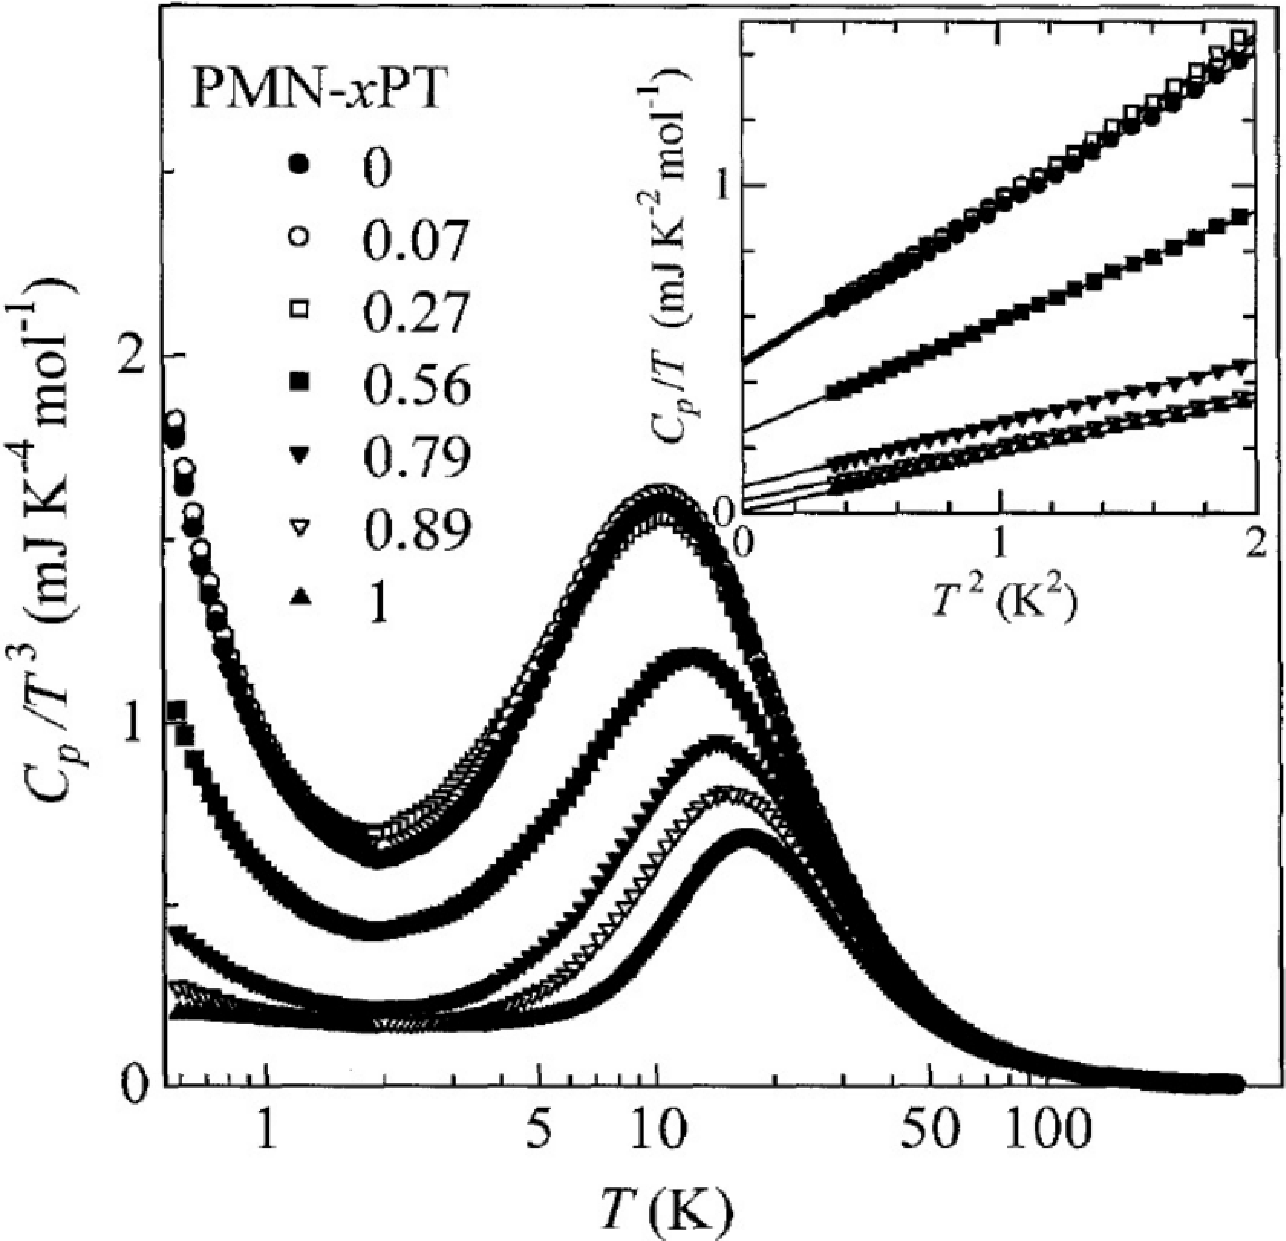
\includegraphics[clip, width=5cm]{img/relaxor-heat-capacity.pdf}
            \hspace{1.6cm} [B]比熱の温度依存性
          \end{center}
        \end{minipage}
        \begin{minipage}{0.5\hsize}
          \begin{center}
            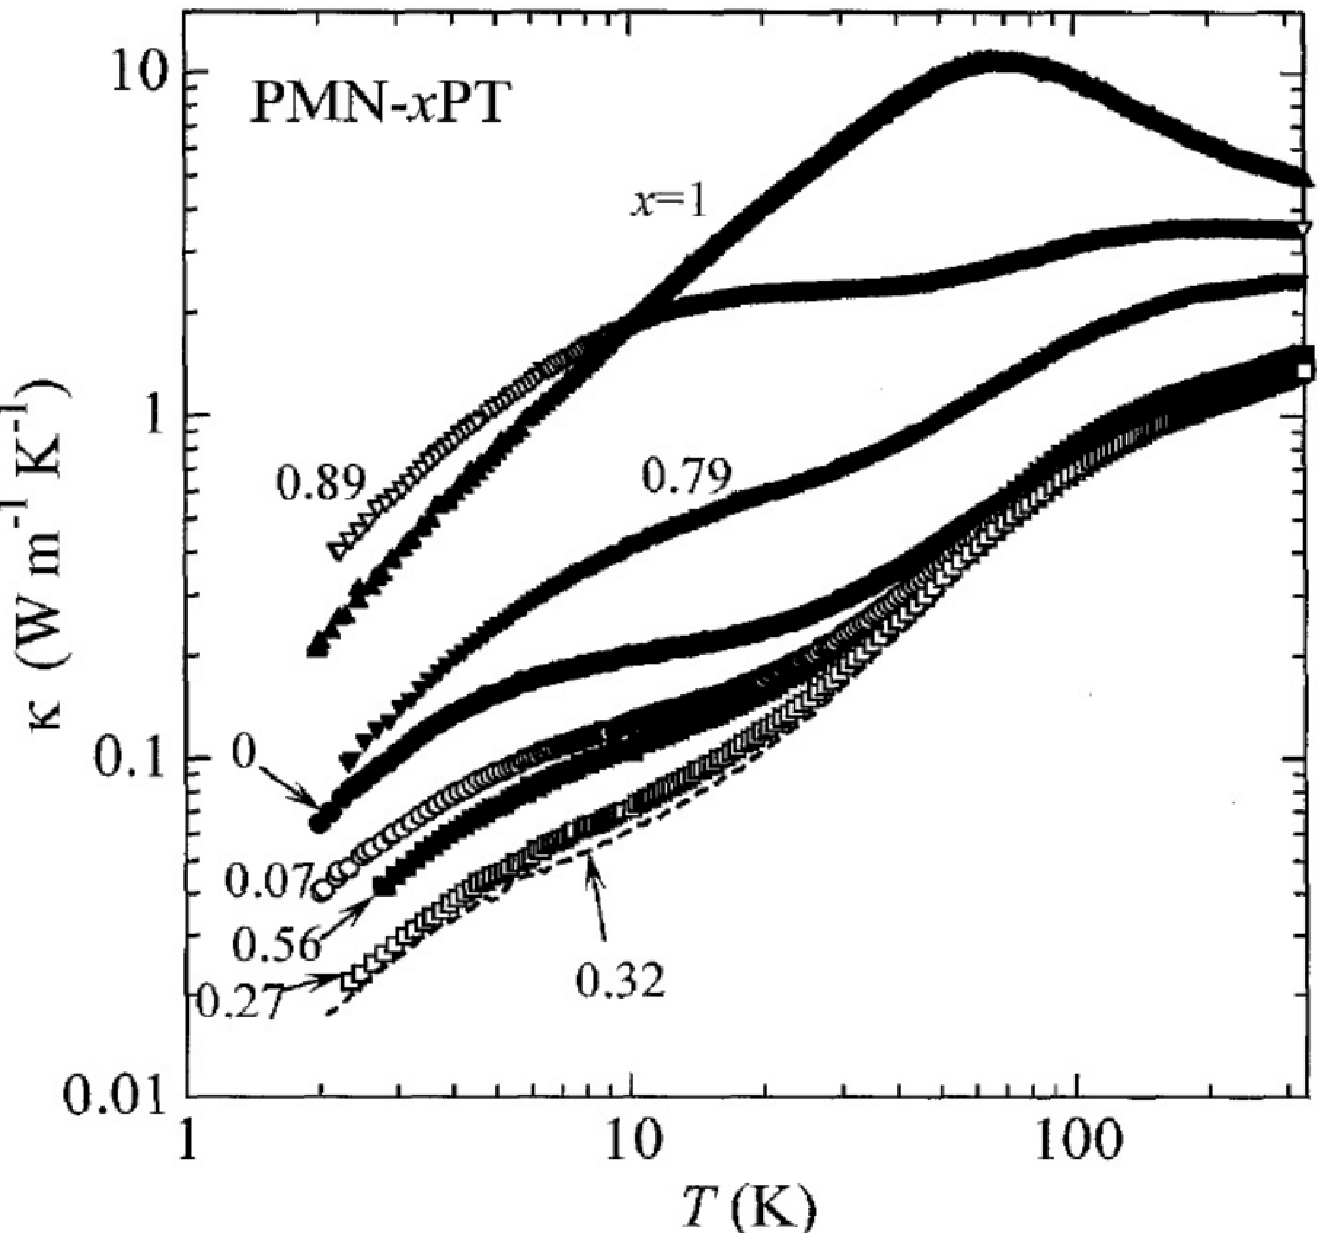
\includegraphics[clip, width=5cm]{img/relaxor-thermal-conductivity.pdf}
            \hspace{1.6cm} [A]熱伝導率の温度依存性
      \end{center}
      \end{minipage}
      \end{tabular}
      \caption{PMN-$x$PTのガラス的な熱物性\cite{relaxCT}}
      \label{fig:lena}
  \end{center}
\end{figure}
僕の研究はこの物質の構造や振動がどうなっているのかを実験して調べるといったことをやっています。最近の研究で、この物質は図\ref{fig:lena}に示しているような温度変化を示すト報告されています。詳しく知りたい人は参考文献\cite{relaxCT}の論文を何とかゲットして読んでみてください。このグラフの意味はここでは詳しくは話しませんが、リラクサーの代表例であるマグネシウムニオブ酸鉛($\rm{Pb(Mg_{1/3}Nb_{2/3})O_3}$, PMN)と普通の強誘電体チタン酸鉛($\rm{PbTiO_3}$, PT)との混ぜ物であるPMN-$x$PTの単結晶についての熱物性を測定したグラフです。このグラフで見比べてほしいのは、$x = 0$のPMNのみの時と、$x = 1$の時のPTのグラフです。ちょっと見にくいですが、PTの時は極低温(10~K以下)で比熱と熱伝導率が前の章で説明した$T^3$に比例しています。しかし、PMNの場合、そうではなく、$T^2$に比例しています。前の章で単結晶はほとんどの場合デバイの$T^3$則に従うというという話をしたのですがリラクサーという物質はそうではありません。では$T^2$という温度依存性はどういう物質で見える温度依存性なのかというと、ガラスです。ガラスは、大体の家の窓ガラスについていると思います。今ではスマホにもついています。ガラスとは物質の名前ではなくガラスという状態を示すものです。窓ガラスは大体は$\rm{SiO}_2$だと思います。$\rm{SiO}_2$は単結晶にもなります。ガラスという状態は、液体の構造がそのまま固まった状態、つまり、ぐちゃぐちゃに原子が結合している状態です。こんな、ガラスには、その種類によらない物性がいくつもあります。その中の一つが低温の熱物性です。この物理的な起源は、大体わかっていますが、ここでは説明を省きます。リラクサーはこのぐちゃぐちゃな構造を持っているガラスとおんなじ温度依存性を持っています。リラクサーは単結晶です。とても規則的に並んでいるものがぐちゃぐちゃな構造とおんなじ物性を示すということはとても奇妙な話です。\par
このように結晶にも関わらず、ぐちゃぐちゃな構造と同じといった物性はいくつも報告されています。とても地味で日常生活には全く役には立たない情報ですが、その物理的な起源を解決することでもしかしたら将来素晴らしい発見の手助けになったりします。私は歴史の一ページの一文字をかく手助けをするものを研究しています。


\section{終わりに}
固体中の熱の動き特に低温側でどのような温度依存性を持っていく科について考えて来ました。正直今回書いた理論的なところは参考文献に書いてあること抜粋して抜き出してきただけになっています。詳しく知りたいとか本当にそんなことがあるのかと思う人はぜひ参考文献を読んでみてくださいかなり詳しく書いてあるのでおすすめします。
%% 参考文献
\begin{thebibliography}{99}
  \bibitem{ondo} \url{https://www.toyo.co.jp/material/products/detail/id=648}
  \item 横田伊佐秋,『物理学テキストシリーズ 熱力学』,岩波書店,1987.
  \item 矢口裕之,『初歩から学ぶ固体物理学』,講談社,2017.
  \item W.COCHRAN・小林正一・福地充(訳),『固体物性シリーズ3 格子振動』,丸善出版,昭和50年.
  \item 田崎晴明,『新物理学シリーズ37 統計力学』,培風館,2008.
  \item 相沢洋二,『キーポイント熱・統計力学』,岩波書店,1996.
 \bibitem{relaxCT}
  Tachibana et al, Appl. Phys. Lett, 93, 092902 (2008).
\end{thebibliography}

\end{document}
%
% ファイトだよ!
%